\documentclass[12pt]{ctexart}%{article}
%\usepackage{zh_CN-Adobefonts_external} % Simplified Chinese Support using external fonts (./fonts/zh_CN-Adobe/)
% fonts
\usepackage[scaled=0.92]{helvet}   % set Helvetica as the sans-serif font
\renewcommand{\rmdefault}{ptm}     % set Times as the default text font

% dmb: not mandatory, but i recommend you use mtpro for math fonts.
% there is a free version called mtprolite.

% \usepackage[amssymbols,subscriptcorrection,slantedGreek,nofontinfo]{mtpro2}

\usepackage[T1]{fontenc}
\usepackage{amsmath}
\usepackage{amsfonts}

% page numbers
\usepackage{fancyhdr}
\fancypagestyle{newstyle}{
\fancyhf{} % clear all header and footer fields
\fancyfoot[R]{\vspace{0.1in} \small \thepage}
\renewcommand{\headrulewidth}{0pt}
\renewcommand{\footrulewidth}{0pt}}
\pagestyle{newstyle}

% geometry of the page
\usepackage[top=1in, bottom=1in, left=1.625in, right=1.625in]{geometry}

% paragraph spacing
\setlength{\parindent}{0pt}
\setlength{\parskip}{2ex plus 0.4ex minus 0.2ex}

% useful packages
\usepackage{natbib}
\usepackage{epsfig}
\usepackage{url}
\usepackage{bm}


\begin{document}

\begin{center}
  \Large \textbf{教育大数据协作计算平台用户指南} \\
  \vspace{0.1in}
  \normalsize 国际应用数据科学研究院 \\
  \today
\end{center}

\tableofcontents
\newpage

\section {教育大数据协作计算平台简介}
教育大数据协同计算平台是云操作系统,它通过数据中心有效管理云系统中的计算资源,存储资源和网络资源。协同计算平台给予管理员和用户不同的权限,云平台管理员通过基于网页浏览器的表格形式管理系统资源,然而普通用户则通过网页浏览器使用资源。协同计算平台主要是为了能够同时让不同用户执行不同任务在同一个系统云平台上协调工作,互不干扰。教育大数据协同计算平台的基本功能: \\
(1) 大数据科研和开发:用户可以在该平台上开展大数据研究和开发,用户可以按照需求安装所需软件和环境,就像在自己的计算机上一样,不同的是用户可以使用所需要的计算资源; \\
(2) 大数据教学:教师可以为一个班级中的每一个学生开一个账号,每一个学生可以安装自己的软件环境,而无需担心影响其他学生,并且每一个学生都可以用所需的计算资源; \\
(3) 高性能计算服务:对于计算密集型的高性能计算应用问题,用户更关心计算效率,如果系统安装有高性能网络,该平台可以将高性能网络与高性能计算任务关联在一起达到高性能的目的; \\
(4) 计算资源社会服务:如果系统具有外部网络,该系统可以对外部用户提供大数据处理和存储服务,也可以为用户提供高性能计算服务; \\
(5) 各种数据库、编译环境、应用软件可根据用户需求进行定制。\\
教育大数据协同计算平台的系统架构如下图\ref{fig:architecture}。

\begin{figure}[!htb]
\centering
\includegraphics[width=5in]{./figures/ArchitectureOfPlatform.png}
%\includegraphics[height=2.1338in, width=3.3307in]{./the_directed_neighbor_tree.png}
%\epsfig{file=./Fig1.png,height=2.1338in, width=3.3307in}
\caption{大数据教育协作计算平台架构}
\label{fig:architecture}
\end{figure}
其功能模块解释如下:
\begin{itemize}
\item 云系统安装/恢复模块:该模块为一个新的系统提供整个系统(一个或多个云系统)的软件安装;如果系统因为某种原因被破坏,该模块提供快速的系统恢复。
\item 系统管理节点/模块:主要用于该系统的软硬件管理、用户管理、任务管理等。
\item 防火墙:如果系统用于对外服务,就需要有外网,外网的安全性需要依靠该防火墙提供。防火墙的种类很多,可根据用户需求选择。
\item 外网:外网服务可以从本地服务商购买,带宽由实际需求决定。
\item 校园网:该系统是在校园网内,校园网的安全由校园网的防火墙提供,该系统没有必要专门为校园网提供防火墙模块。
\item IPMI模块:该模块为系统管理提供服务,它甚至可以在关机状态下提供远程开关机服务等。
\item 高速网络模块:该模块提供计算和存储节点之间的快速数据交换。对于高性能计算或者其他需要快速数据交换的网络时,该模块提供高速数据交换。
\item 系统管理交换模块:该模块负责计算节点之间、存储节点之间以及计算节点与存储节点之间的数据交换。
\item 计算节点:该模块负责任务计算,每个模块具有CPU和GPU计算单元服务不同大数据研发和教学任务。
\end{itemize}
教育大数据协同计算平台功能列表:

\begin{table*}[!htb]
\centering
\caption{教育大数据协作计算平台功能列表}  \label{table1}
\begin{tabular}{|c|c|} \hline
1 & 协同计算安装和恢复模块 \\ \hline
2 & 协同计算平台管理模块   \\ \hline
3 & 协同计算应用仓库     \\ \hline
4 & 协同计算用户管理系统  \\ \hline
5 & 协同计算任务管理系统  \\ \hline
6 & 协同计算大数据开发环境 \\ \hline
7 & 协同计算并行管理系统   \\ \hline
8 & 协同计算大数据架构系统  \\ \hline
9 & 协同计算存储系统 \\ \hline
10 & 协同计算网络环境系统  \\ \hline
\end{tabular}
\end{table*}

\section {协同计算安装和恢复模块}
需要补充
\section{协同计算平台管理模块}
在使用本指南之前,用户需要向所在单位网络运营管理部门申请IP地址和域名,为后续运营管理该协作计算平台做好准备工作。
\subsection{登陆管理平台}
打开浏览器,输入协作管理平台IP地址XXX.XXX.XXX.XXX或域名www.xxx.xxx.com,回车,得到如图\ref{fig:login}所示登陆界面。

\begin{figure}[!htb]
\centering
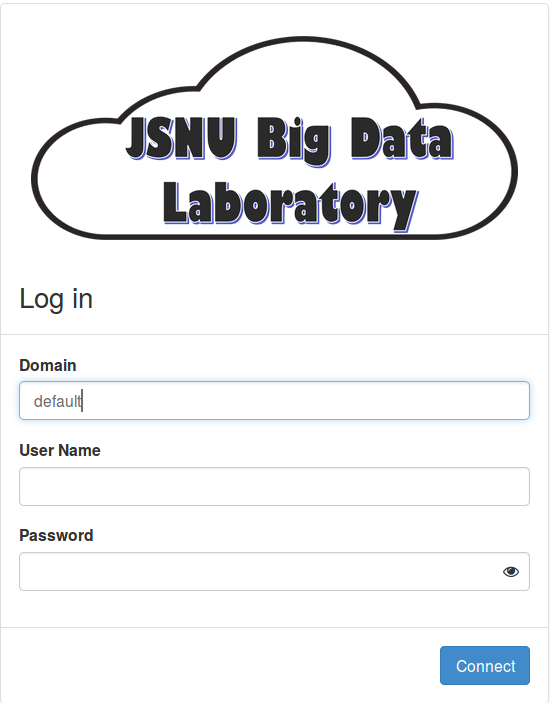
\includegraphics[width=5in]{./figures/login}
%\includegraphics[height=2.1338in, width=3.3307in]{./the_directed_neighbor_tree.png}
%\epsfig{file=./Fig1.png,height=2.1338in, width=3.3307in}
\caption{登陆界面}
\label{fig:login}
\end{figure}
在该页面需要用户输入域名(\textbf{domain})、用户名(\textbf{user name})以及密码(\textbf{password})。这里域名跟上面提到域名不同,用户只需要输入\textbf{default}即可,用户名和密码则为协作平台管理员为不同用户分配的用户名和密码。输入完毕,点击\textbf{Sign In},进入协作平台管理界面如图\ref{fig:identityprojects}。如果以普通用户身份登陆系统,该页面只显示项目选项(\textbf{Project});如果以管理员身份登陆,该页面显示项目选项(\textbf{Project})、管理选项(\textbf{Admin})以及标识选项(\textbf{Identity})。
管理界面只有管理员能够看到,其它用户无法查看。管理界面综合展示了系统资源的管理与使用情况如图\ref{fig:adminsystemoverview},包括系统超级管理、卷管理、网络以及镜像等。其中``Overview''显示了不同项目使用系统资源情况,用户可以按指定时间段进行查看。
\begin{figure}[!htb]
\centering
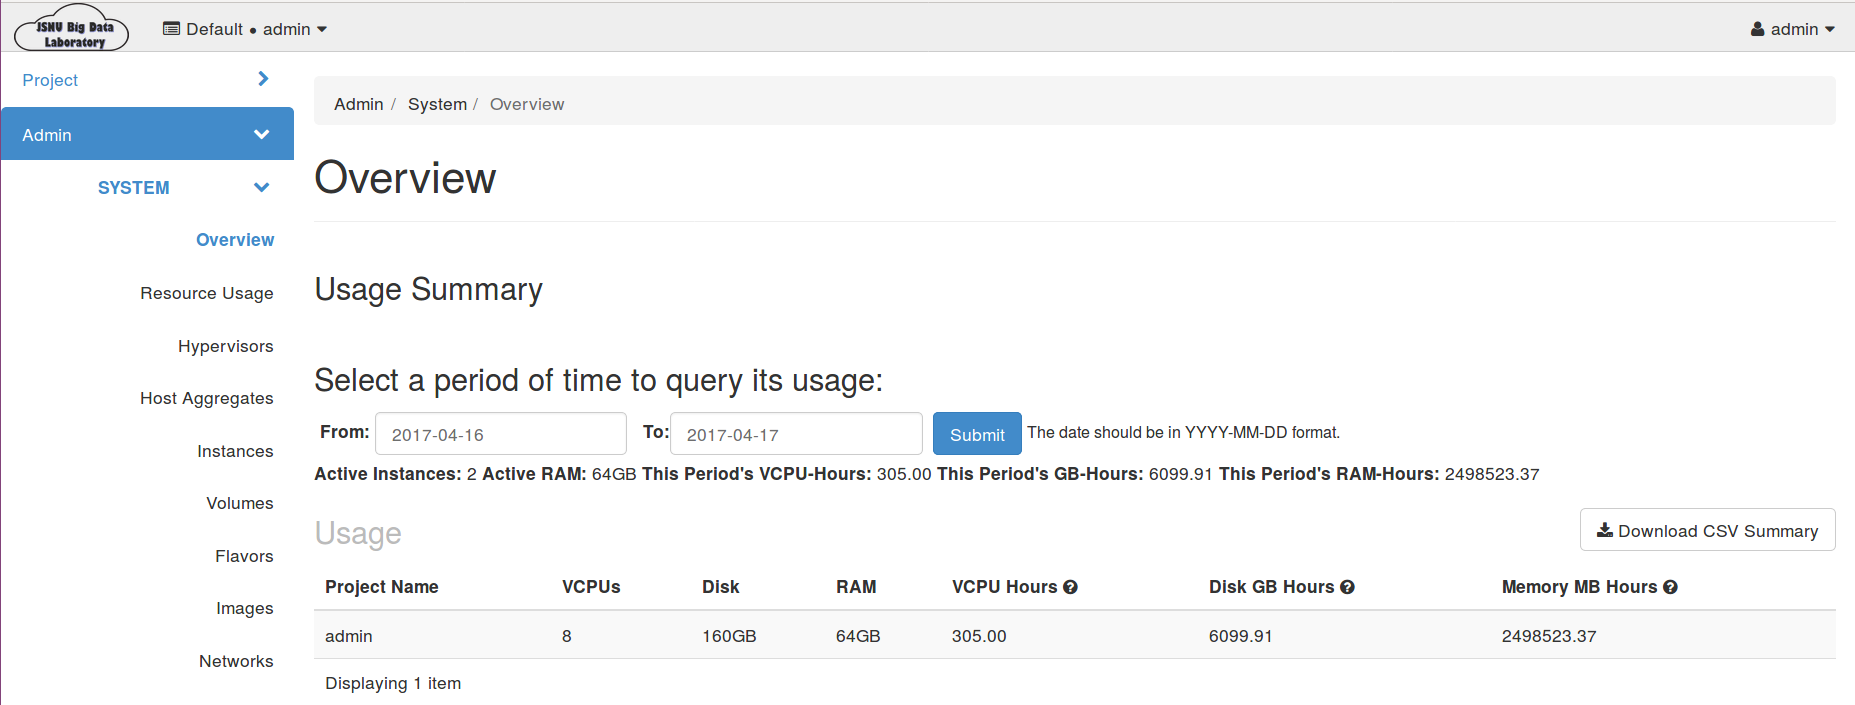
\includegraphics[width=6in]{./figures/Admin_System_Overview}
%\includegraphics[height=2.1338in, width=3.3307in]{./the_directed_neighbor_tree.png}
%\epsfig{file=./Fig1.png,height=2.1338in, width=3.3307in}
\caption{协作平台管理界面}
\label{fig:adminsystemoverview}
\end{figure}

``Hypervisors''界面列出了系统超级管理器,包括各计算节点资源利用情况、运行状态等。图\ref{fig:adminsystemhypervisors}中``Hypervisor''按钮列出了平台各计算节点资源配置情况,包括虚拟内核数量、内存、硬盘等,
\begin{figure}[!htb]
\centering
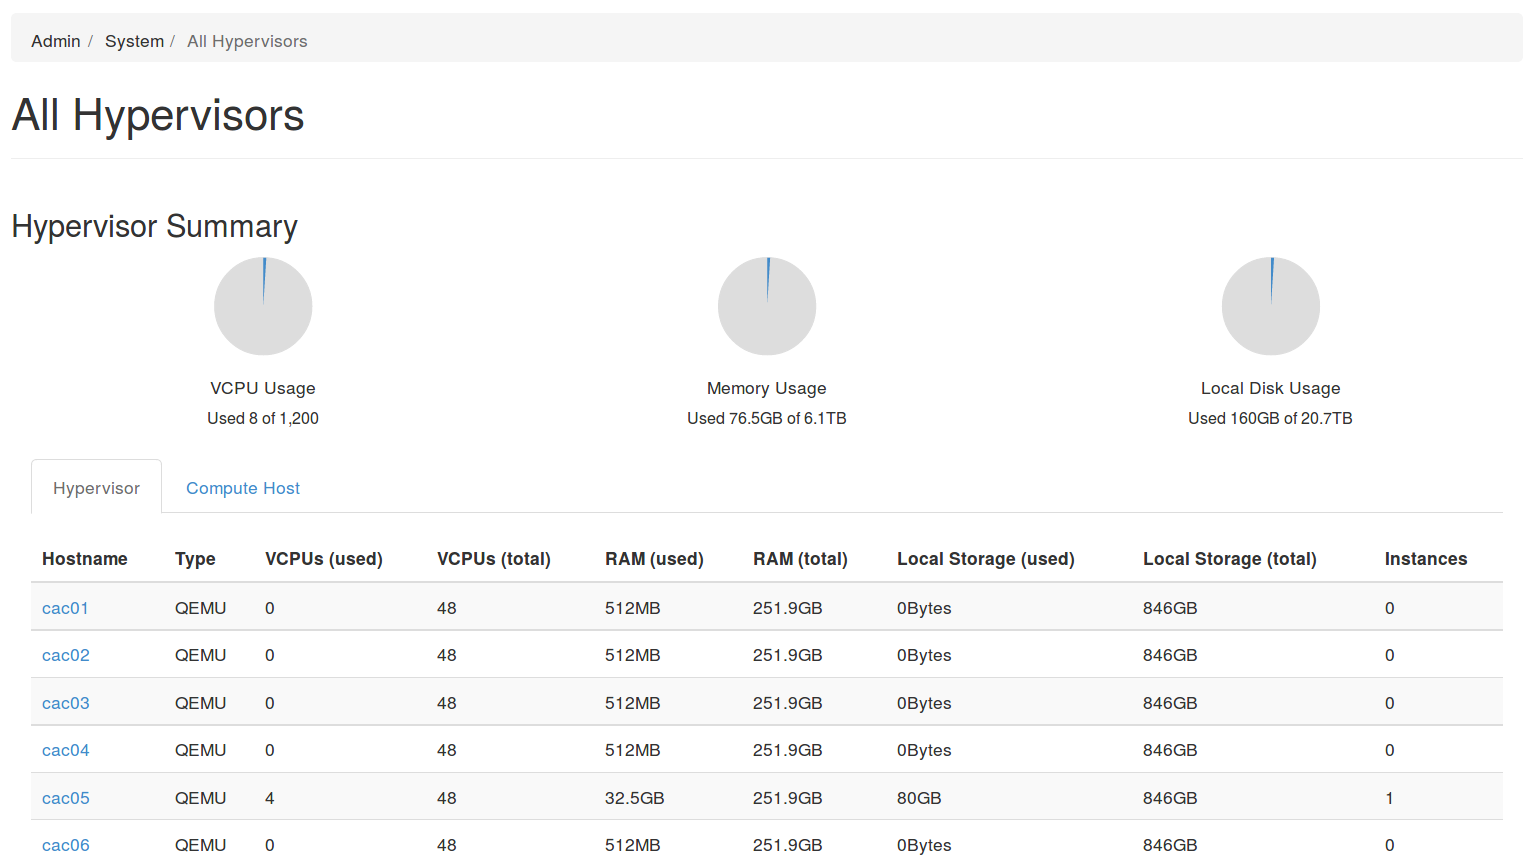
\includegraphics[width=6in]{./figures/Admin_System_Hypervisors}
\caption{协作平台超级管理器}
\label{fig:adminsystemhypervisors}
\end{figure}

``Host Aggregates'' 如图\ref{fig:adminsystemhostagregates}是在 Availability Zones 的基础上更进一步地进行逻辑的分组和隔离。例如我们可以根据不同的 computes 节点的物理硬件配置将具有相同共性的物理资源规划在同一 Host Aggregate 之下,或者根据用户的具体需求将几个 computes 节点规划在具有相同用途的同一 Host Aggregate 之下,通过这样的划分有利于提高 OpenStack 资源的使用效率。Host Aggregates 可以通过 nova client 或 API 来创建和配置。Availability Zones 通常是对 computes 节点上的资源在小的区域内进行逻辑上的分组和隔离。例如在同一个数据中心,我们可以将 Availability Zones 规划到不同的机房,或者在同一机房的几个相邻的机架,从而保障如果某个 Availability Zone 的节点发生故障(如供电系统或网络),而不影响其他的 Availability Zones 上节点运行的虚拟机,通过这种划分来提高 OpenStack 的可用性。目前 OpenStack 默认的安装是把所有的 computes 节点划分到 nova 的 Availability Zone 上,但我们可以通过对 nova.conf 文件的配置来定义不同的 Availability zones。
\begin{figure}[!htb]
\centering
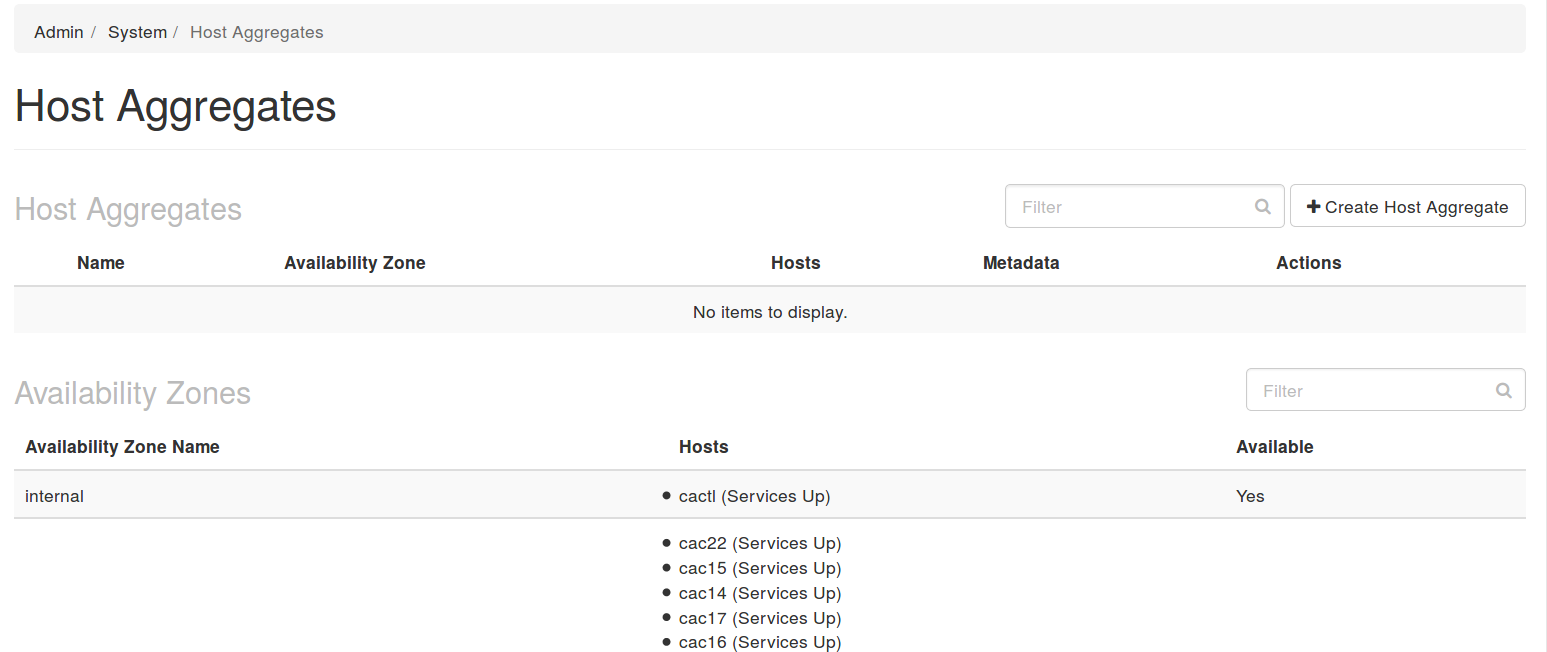
\includegraphics[width=6in]{./figures/Admin_System_HostAggregates}
\caption{协作平台主机汇聚管理}
\label{fig:adminsystemhostagregates}
\end{figure}
``Instance''如图\ref{fig:adminsysteminstances}显示当前在写作平台运行的对象的相关信息,如所在节点、名称、镜像、IP地址以及配额等。用户可以在``Instance''界面编辑对象、删除对象。
\begin{figure}[!htb]
\centering
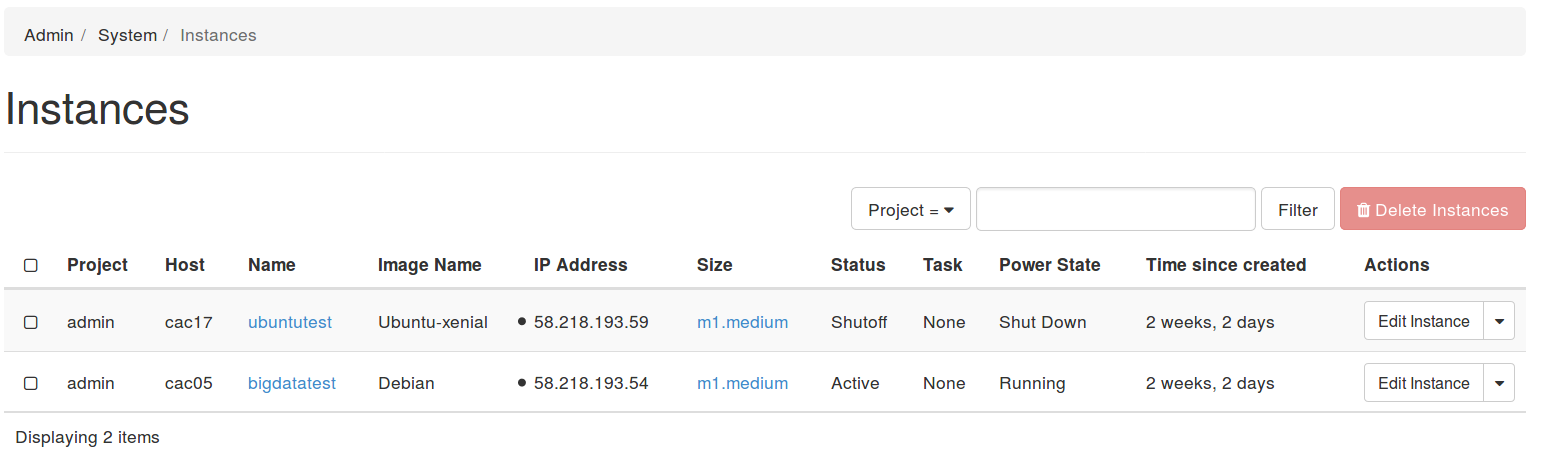
\includegraphics[width=6in]{./figures/Admin_System_Instances}
\caption{协作平台对象管理界面}
\label{fig:adminsysteminstances}
\end{figure}
``Volumes''如图\ref{fig:adminsystemvolumes}主要用于卷管理,其中``Volumes''子界面列出了当前不同项目卷的基本信息,``Volume Types''列出不同卷类型信息,``Volume Snapshots''显示卷快照信息。
\begin{figure}[!htb]
\centering
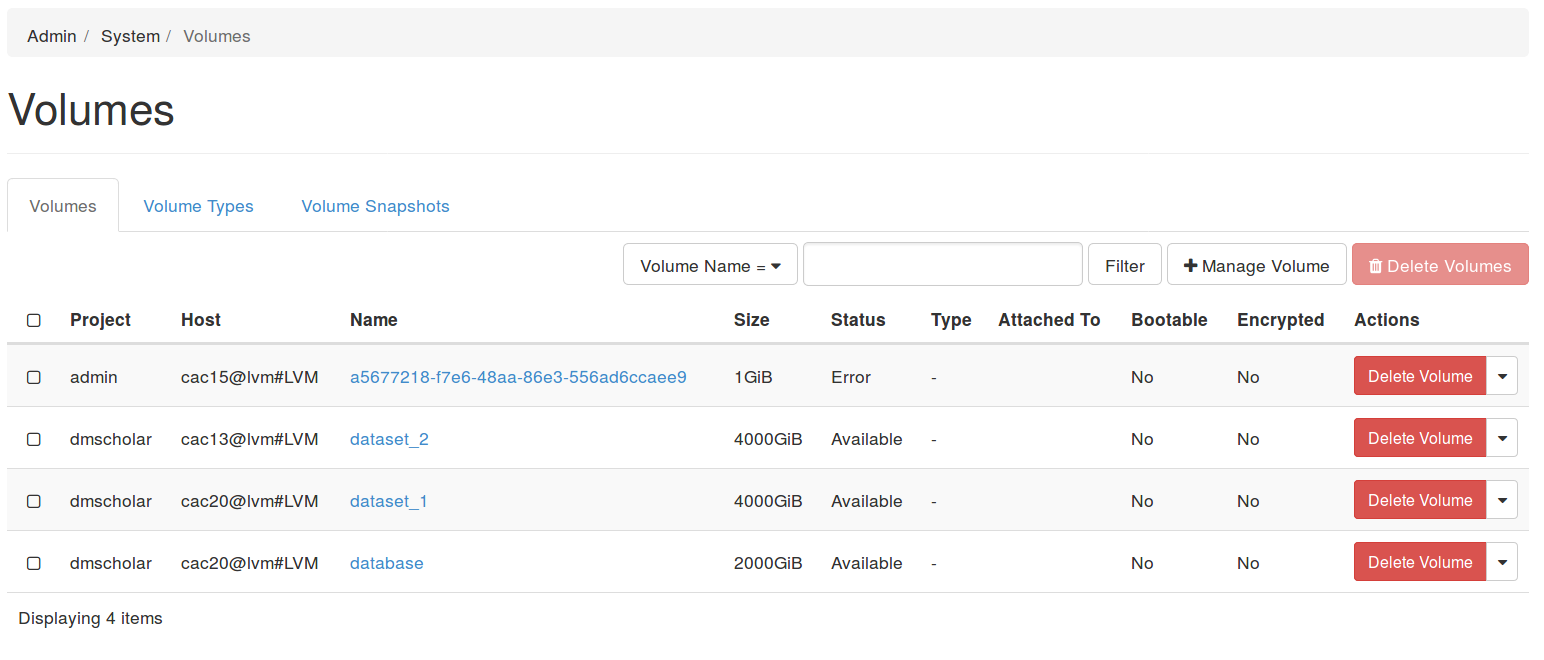
\includegraphics[width=6in]{./figures/Admin_System_Volumes}
\caption{协作平台卷管理界面}
\label{fig:adminsystemvolumes}
\end{figure}
``Flavors''如图\ref{fig:adminsystemflavors}为用户定制了不同对象模板,他们对资源占用情况不同。用户可以根据特定应用场景选择合适的模板创建对象。用户可以通过``+Create Flavor''定制模板,可以通过对应模板右侧下拉菜单对模板进行编辑。
\begin{figure}[!htb]
\centering
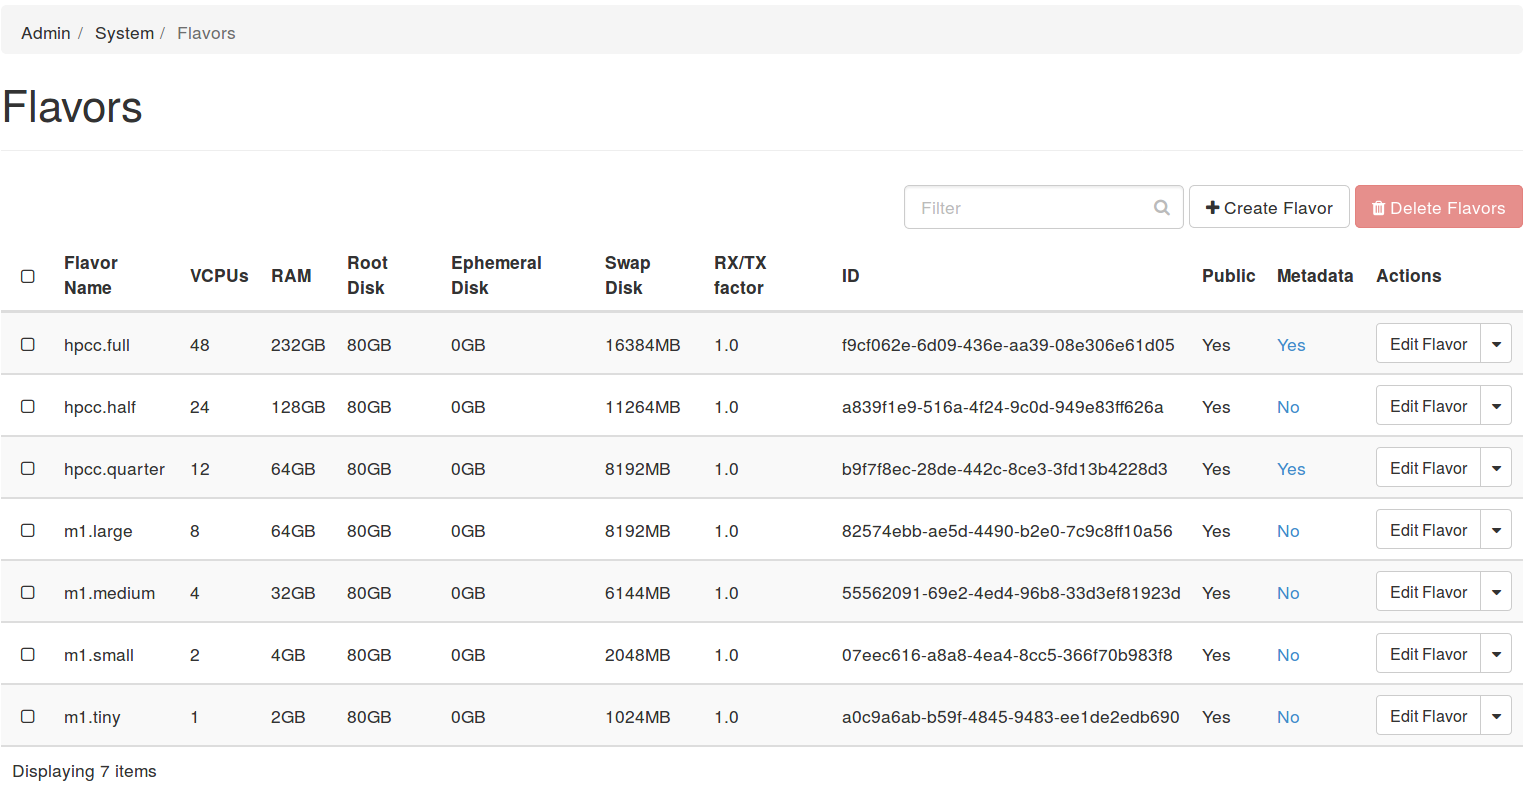
\includegraphics[width=6in]{./figures/Admin_System_Flavors}
\caption{协作平台模板管理界面}
\label{fig:adminsystemflavors}
\end{figure}
``Images''如图\ref{fig:adminsystemimages}为用户提供了镜像管理接口。镜像通常定义了对象所使用的操作系统,是用户创建对象的起始点,用户可以点击镜像右侧下拉菜单创建指定镜像的对象,用户还可以通过``+Create Image''自行创建镜像。
\begin{figure}[!htb]
\centering
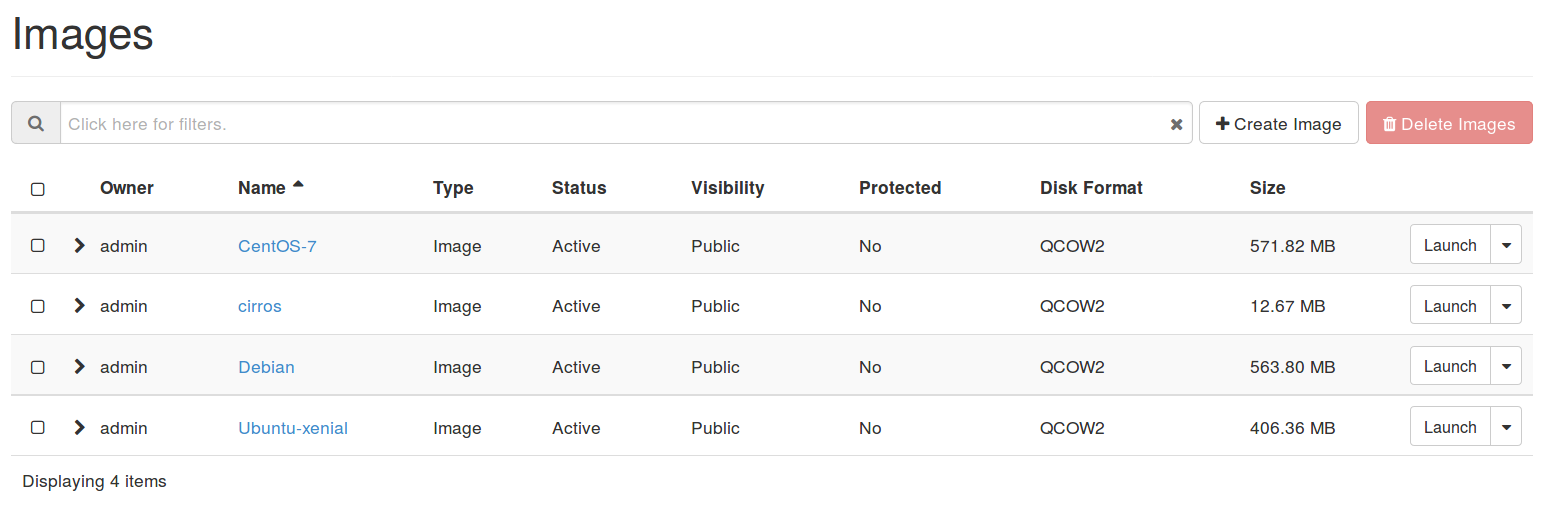
\includegraphics[width=6in]{./figures/Admin_System_Images}
\caption{协作平台镜像管理界面}
\label{fig:adminsystemimages}
\end{figure}
``Networks''如图\ref{fig:adminsystemnetworks}显示不同项目的网络信息以及运行状况。用户可以通过右侧下拉菜单编辑网络,也可以通过``+Create Network''创建网络。
\begin{figure}[!htb]
\centering
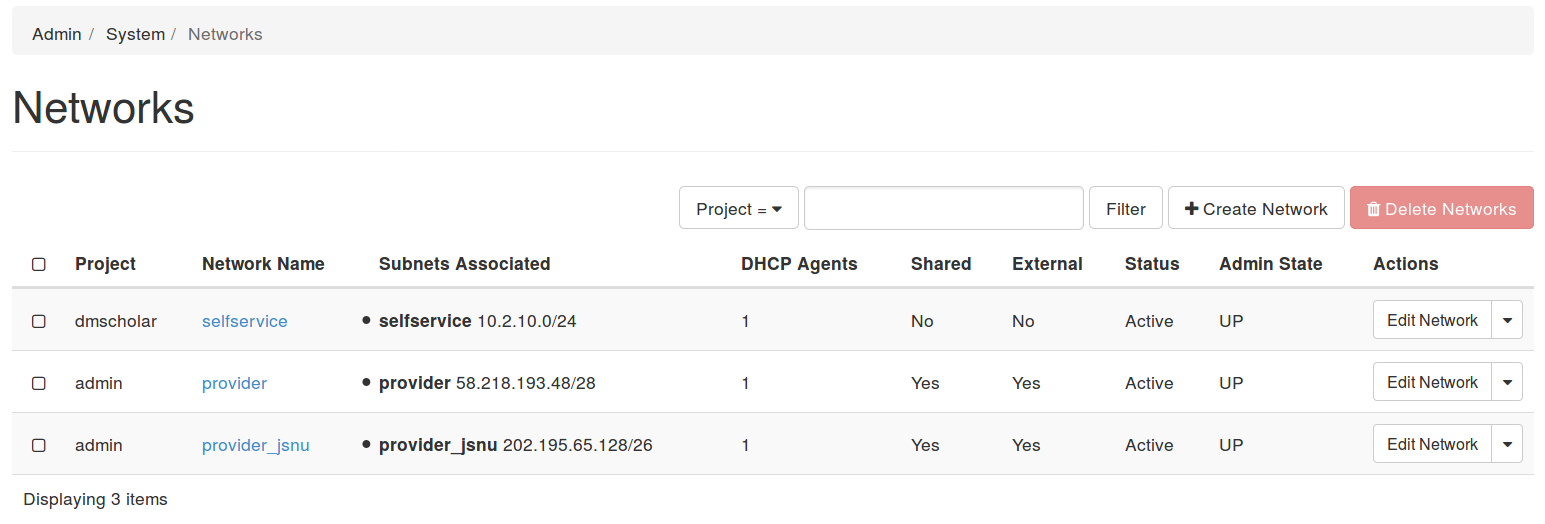
\includegraphics[width=6in]{./figures/Admin_System_Networks}
\caption{协作平台网络管理界面}
\label{fig:adminsystemnetworks}
\end{figure}
``Routers''如图\ref{fig:adminsystemrouters}列出了协作平台不同项目内部的路由信息。
\begin{figure}[!htb]
\centering
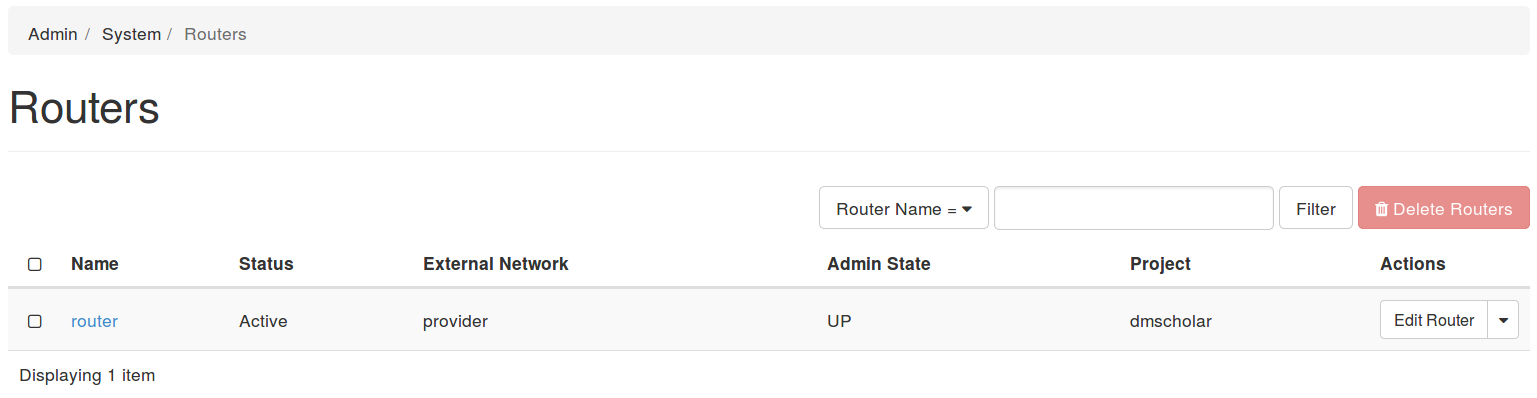
\includegraphics[width=6in]{./figures/Admin_System_Routers}
\caption{协作平台路由管理界面}
\label{fig:adminsystemrouters}
\end{figure}
``Floating IPs''如图\ref{fig:adminsystemfloatingip}列出管理员为不同项目分配的IP地址。管理员可以通过``Allocate IP To Project''为项目分配IP地址,也可以通过右侧``Release Floating IP''释放已分配IP。
\begin{figure}[!htb]
\centering
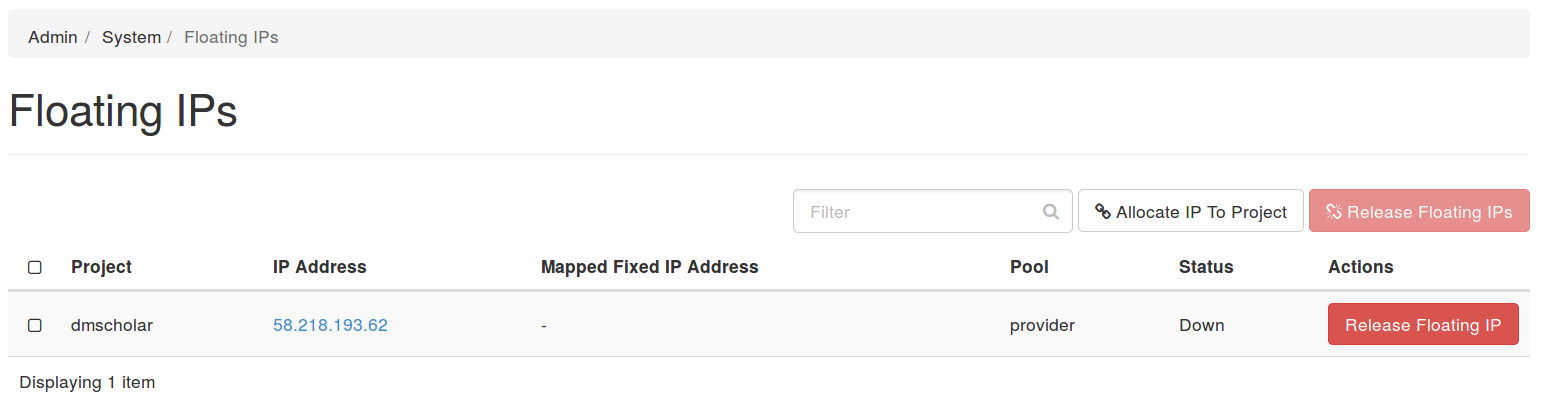
\includegraphics[width=6in]{./figures/Admin_System_FloatingIP}
\caption{协作平台IP地址管理界面}
\label{fig:adminsystemfloatingip}
\end{figure}
``Defaults''如图\ref{fig:adminsystemdefaults}显示了协作平台的默认管理信息,管理员可以查看系统资源使用及管理信息。
\begin{figure}[!htb]
\centering
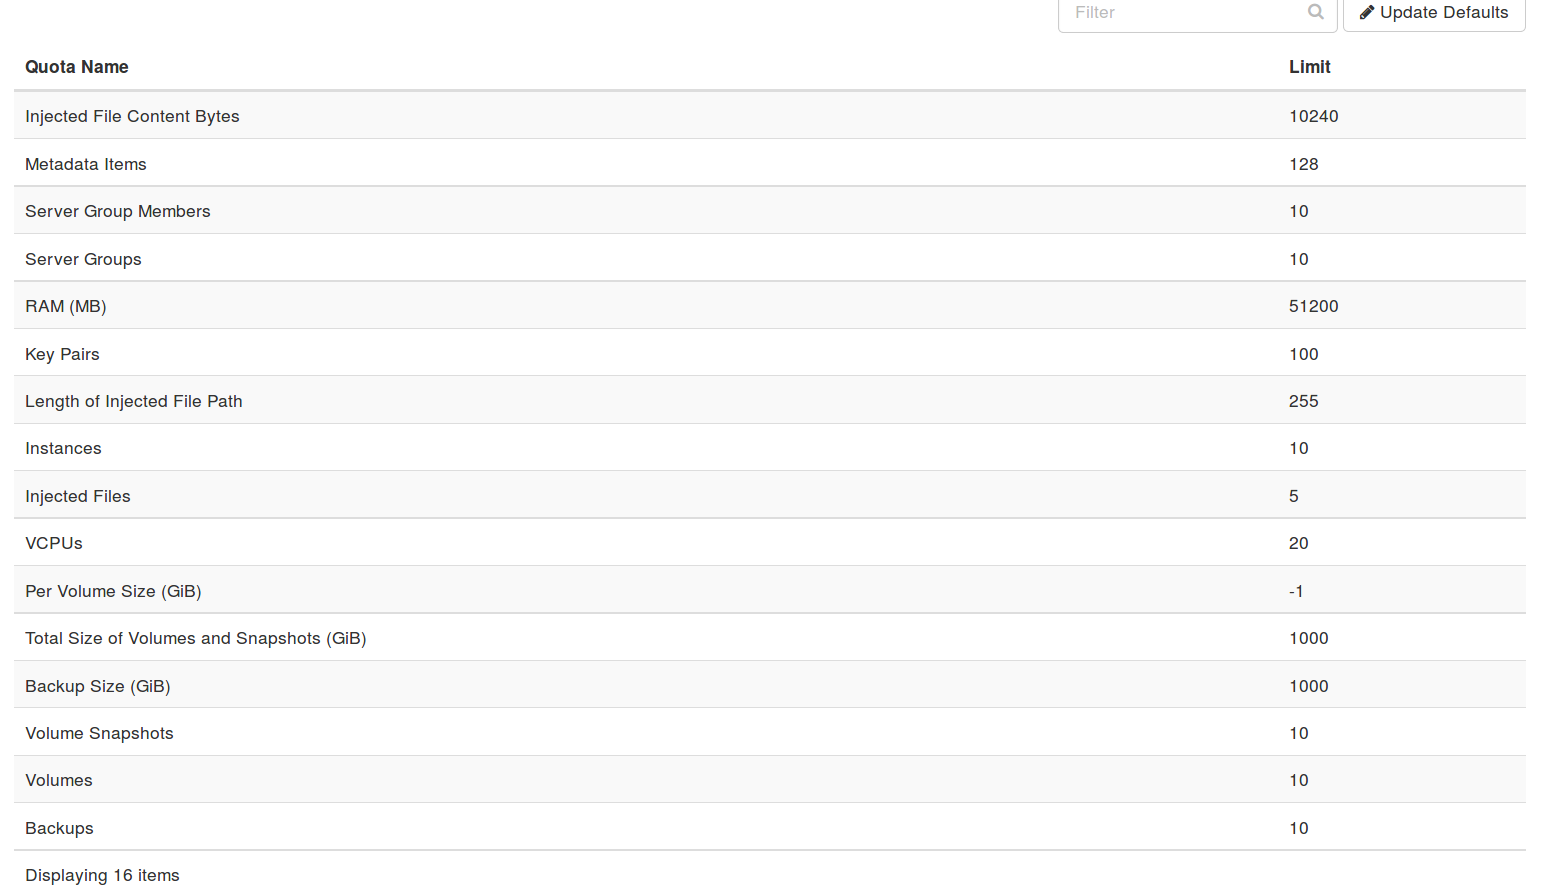
\includegraphics[width=6in]{./figures/Admin_System_Defaults}
\caption{协作平台常规管理信息}
\label{fig:adminsystemdefaults}
\end{figure}

``System Information''如图\ref{fig:adminsystemsysteminformation}所示列出了写作平台所提供的各类服务,例如卷、网络、标识、测量等;``Compute Services''列出了计算服务的详细信息如名称、节点、域以及状态等;``Block Storage Services''显示块存储服务信息,``Network Agents''列出网路服务信息。
\begin{figure}[!htb]
\centering
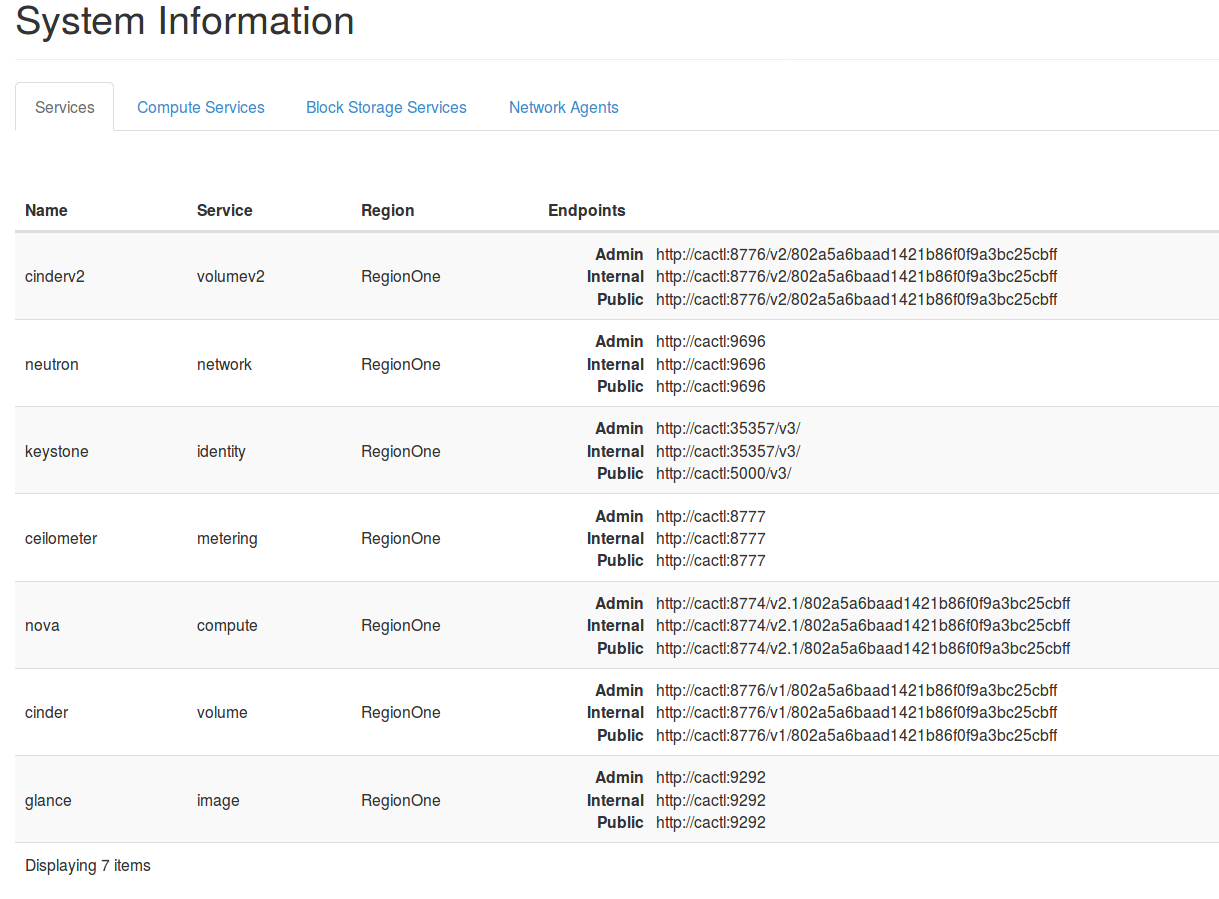
\includegraphics[width=6in]{./figures/Admin_System_SystemInformation}
\caption{协作平台系统管理信息}
\label{fig:adminsystemsysteminformation}
\end{figure}
\section{协同计算应用仓库} 

\section{协同计算用户管理系统}  
用户标识页面显示了协作平台用户信息如图\ref{fig:identityusers}所示,包括用户名、用户描述、用户邮箱、用户ID等,管理用户可以通过用户标识页面管理、创建用户。“+Create User”按钮提供创建用户接口,“Actions”列的下拉菜单提供了管理用户的接口,如删除用户、修改密码等。
\begin{figure}[!htb]
\centering
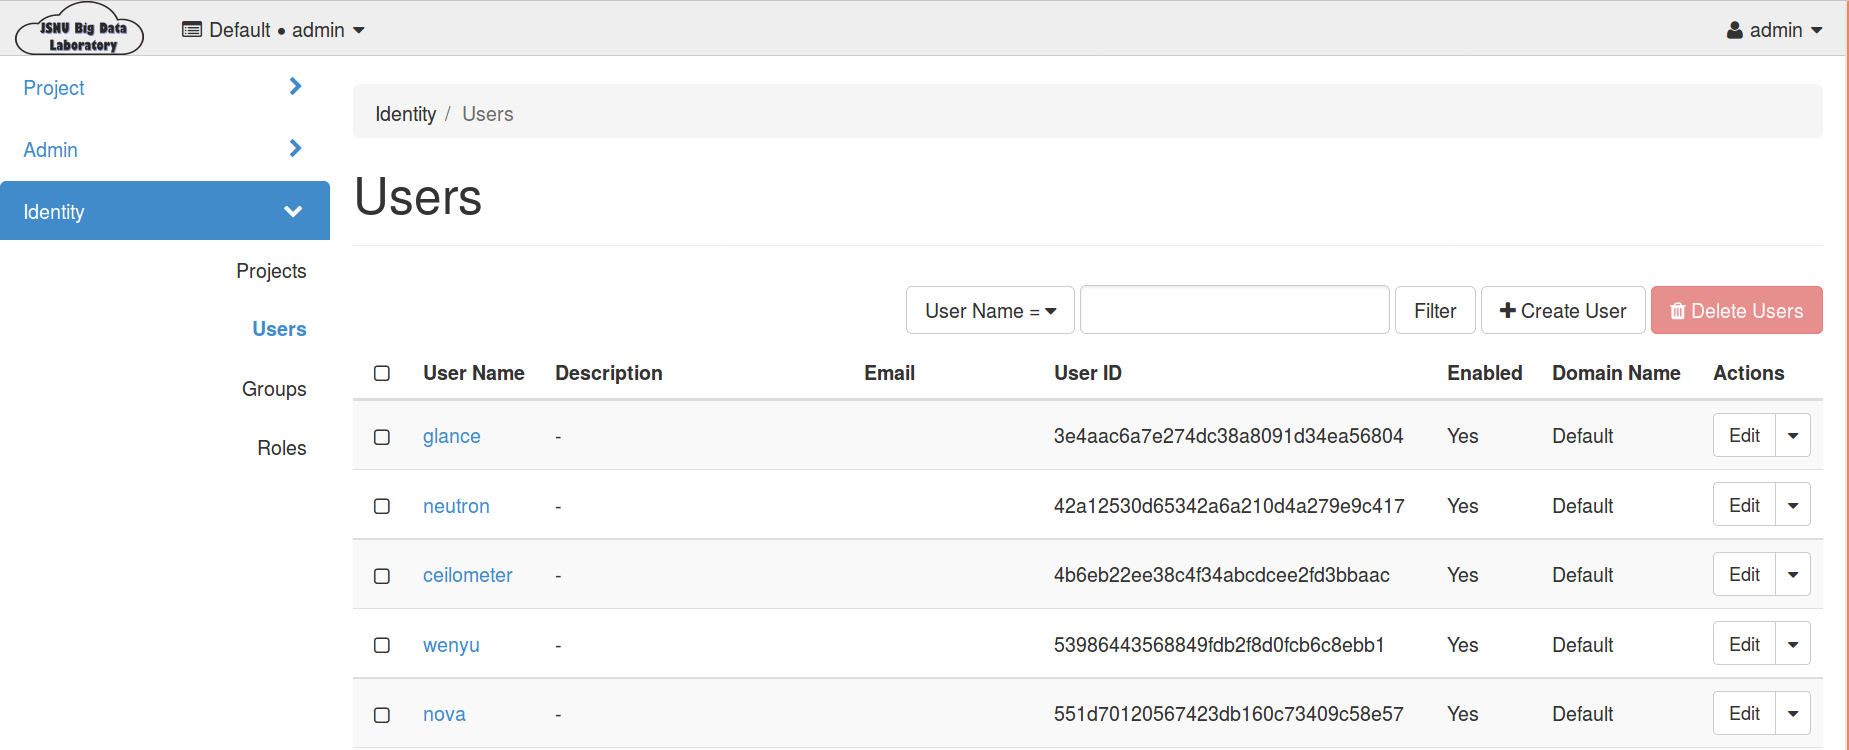
\includegraphics[width=6in]{./figures/Identity_Users}
%\includegraphics[height=2.1338in, width=3.3307in]{./the_directed_neighbor_tree.png}
%\epsfig{file=./Fig1.png,height=2.1338in, width=3.3307in}
\caption{用户标识界面}
\label{fig:identityusers}
\end{figure}
群组主要用来方便管理用户,群组标识如图\ref{fig:identitygroups}列出了当前协作平台已有群组信息,包括名称、描述、ID等,提供了管理群组的接口,如“+Create Group”创建群组、“Actions”编辑群组等。
\begin{figure}[!htb]
\centering
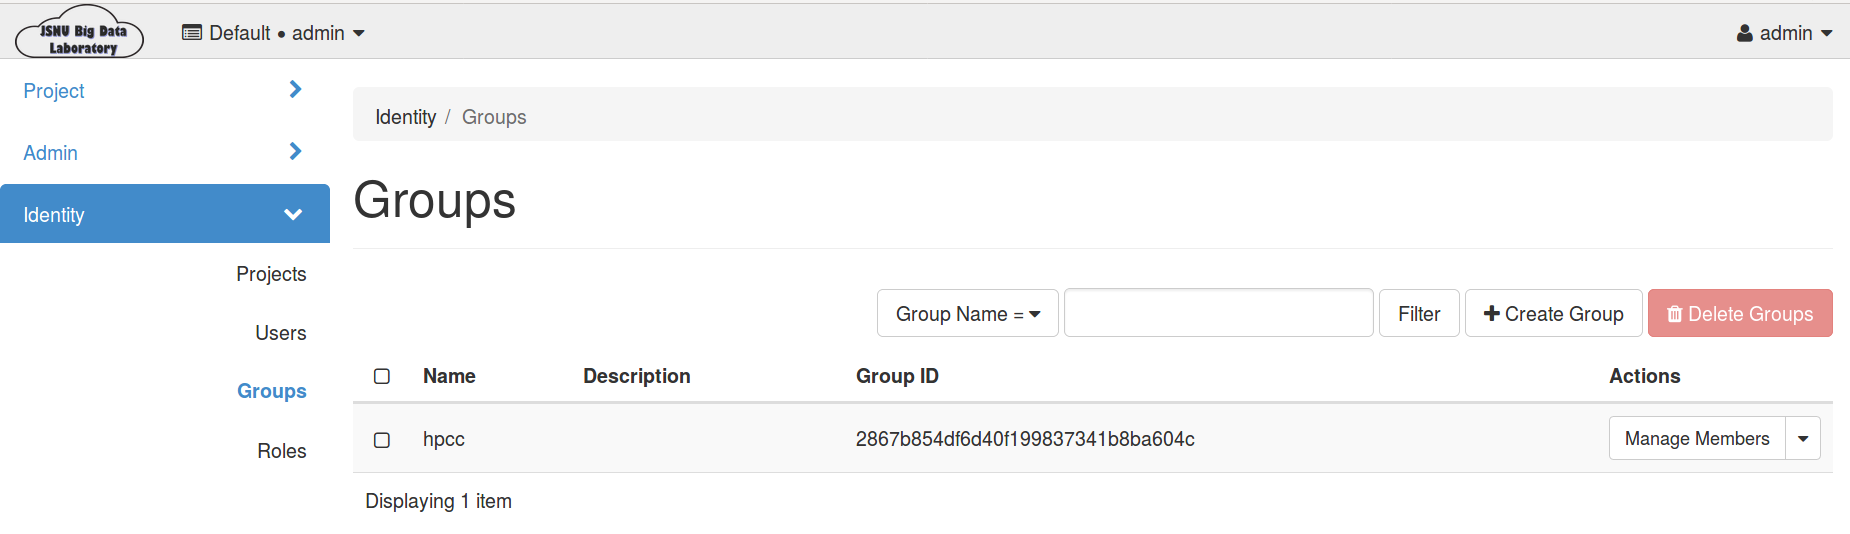
\includegraphics[width=6in]{./figures/Identity_Groups}
%\includegraphics[height=2.1338in, width=3.3307in]{./the_directed_neighbor_tree.png}
%\epsfig{file=./Fig1.png,height=2.1338in, width=3.3307in}
\caption{群组标识界面}
\label{fig:identitygroups}
\end{figure}
角色从宏观层面将用户分类,不同用户拥有不同角色。图\ref{fig:identityroles}角色标识列出了当前平台所提供的角色,如用户、管理员,以及角色ID等。用户可以根据特定需求创建角色。
\begin{figure}[!htb]
\centering
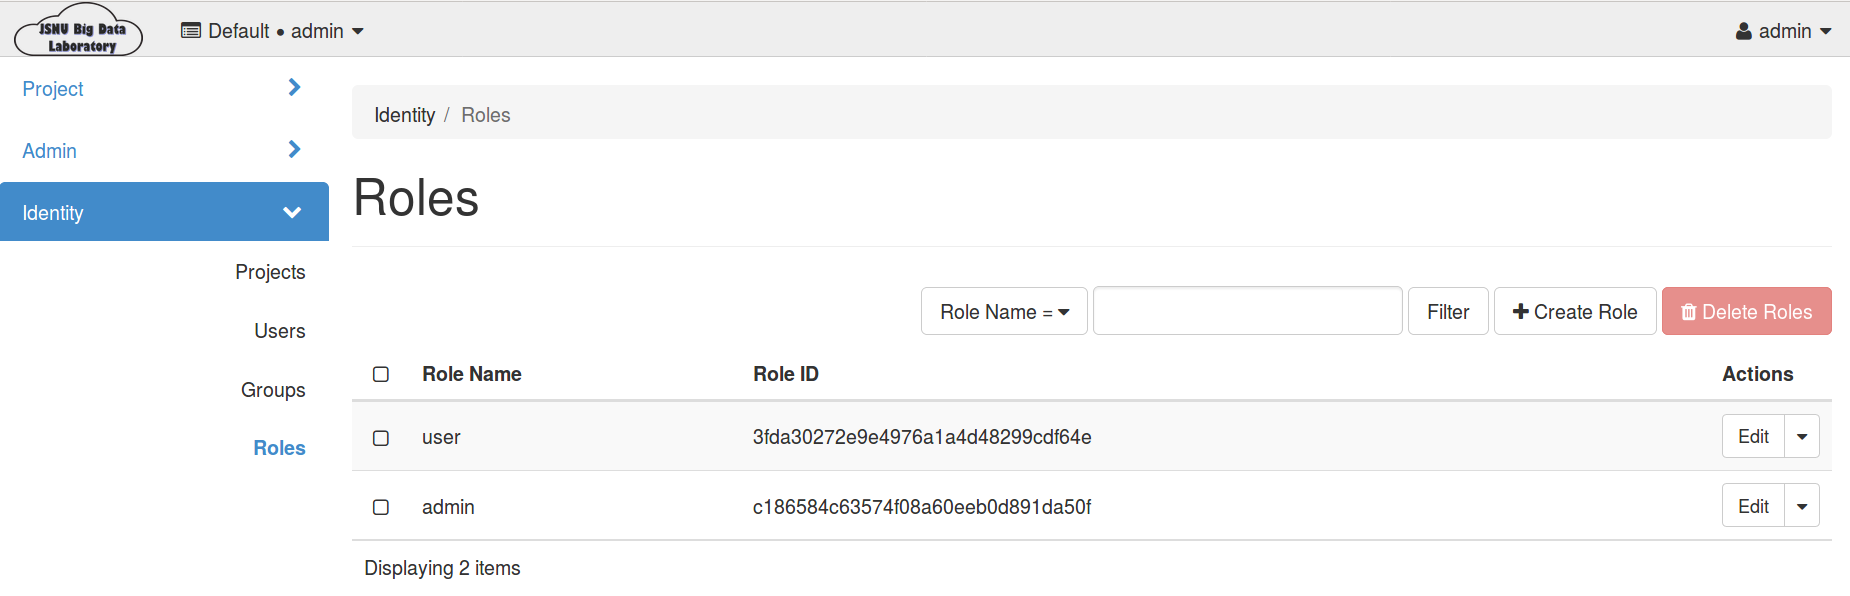
\includegraphics[width=6in]{./figures/Identity_Roles}
%\includegraphics[height=2.1338in, width=3.3307in]{./the_directed_neighbor_tree.png}
%\epsfig{file=./Fig1.png,height=2.1338in, width=3.3307in}
\caption{角色标识界面}
\label{fig:identityroles}
\end{figure}
\subsection{管理}
\section{协同计算任务管理系统} 
``Project''帮助用户管理项目相关信息,主要包括``COMPUTE''计算信息和``NETWORK''网络信息。如图\ref{fig:projectcomputeoverview}为``COMPUTE''总览,显示各类资源使用信息,以及不同对象的资源使用情况。
\begin{figure}[!htb]
\centering
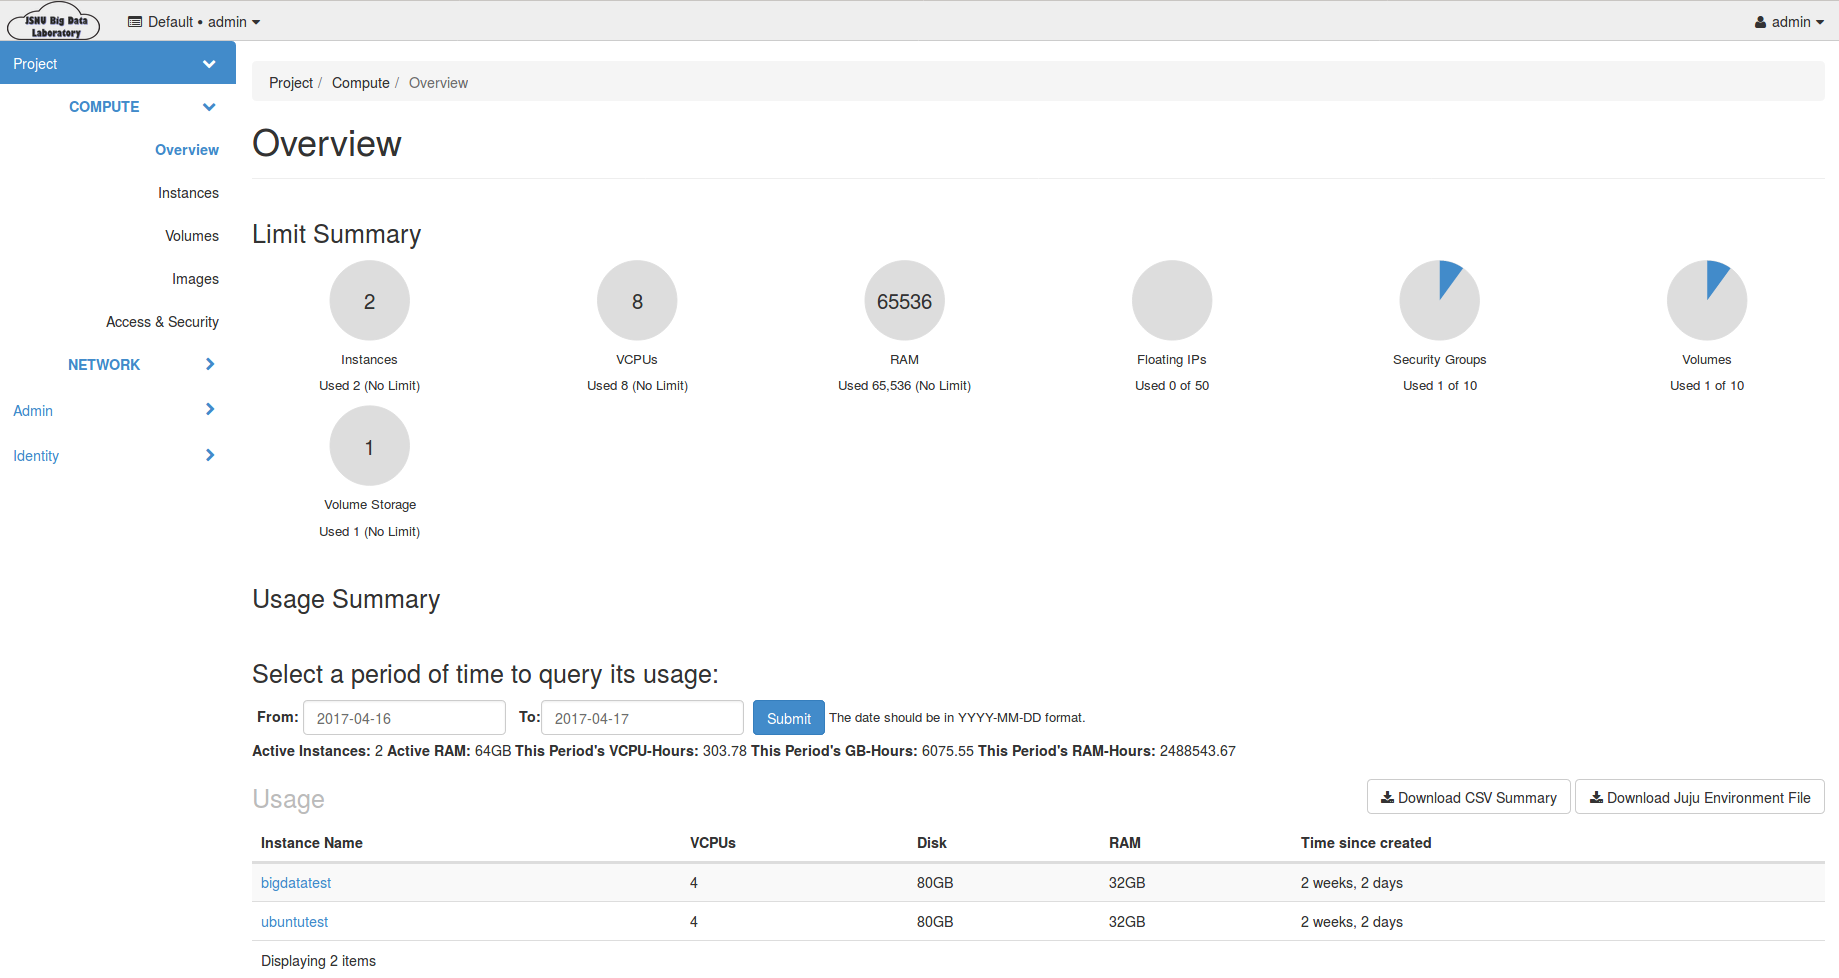
\includegraphics[width=6in]{./figures/Project_Compute_Overview}
\caption{协作平台项目信息总览}
\label{fig:projectcomputeoverview}
\end{figure}
``Instance''如图\ref{fig:projectcomputeinstances}列出了各对象的详细信息包括IP地址、运行状态、镜像等。用户可以通过右上角``Launch Instance''创建对象,还可以通过对象右侧下拉菜单对对象进行管理。
\begin{figure}[!htb]
\centering
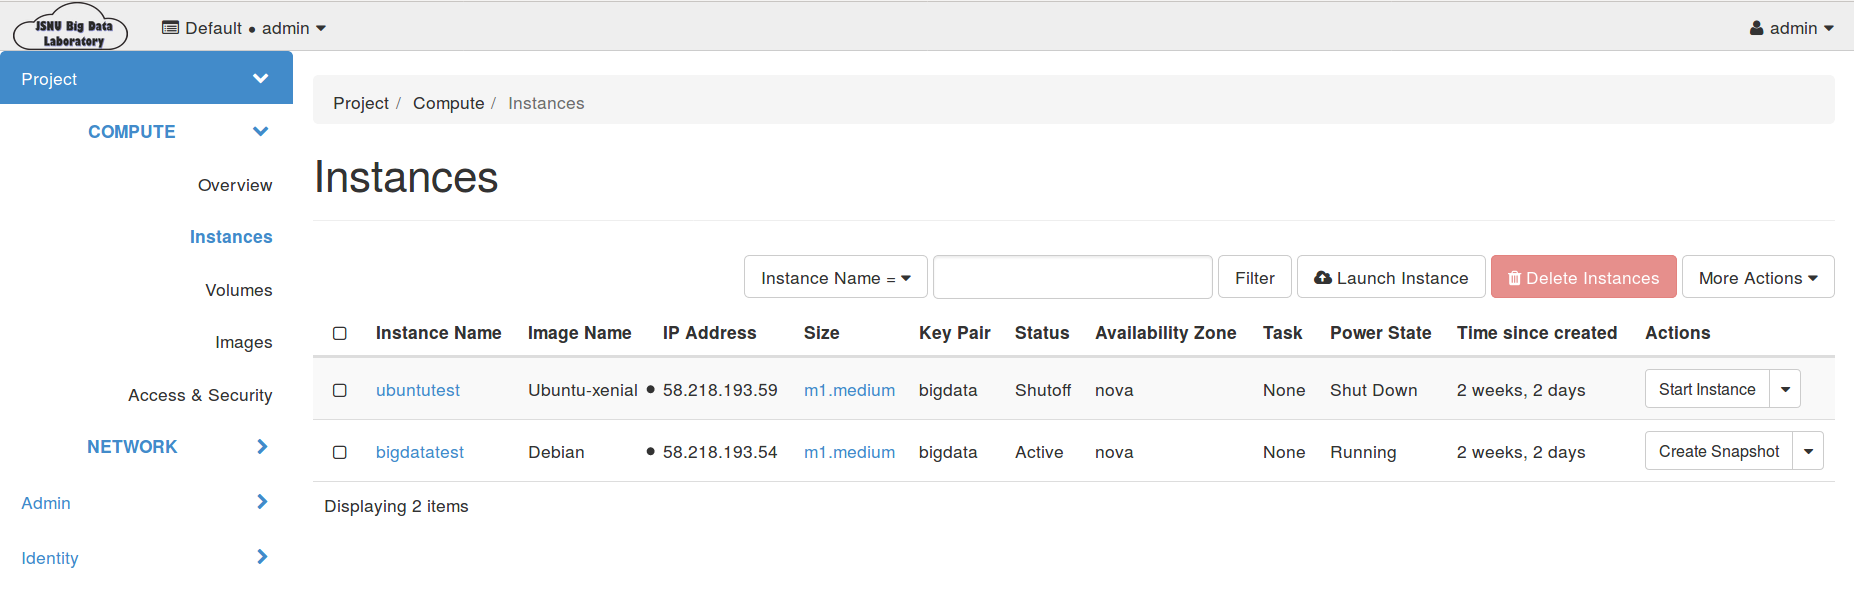
\includegraphics[width=6in]{./figures/Project_Compute_Instances}
\caption{协作平台项目对象}
\label{fig:projectcomputeinstances}
\end{figure}

``Images''列出了镜像详细信息。用户可以通过右上角``+Create Image''创建镜像,可以通过镜像右侧下拉菜单启动对象。
\begin{figure}[!htb]
\centering
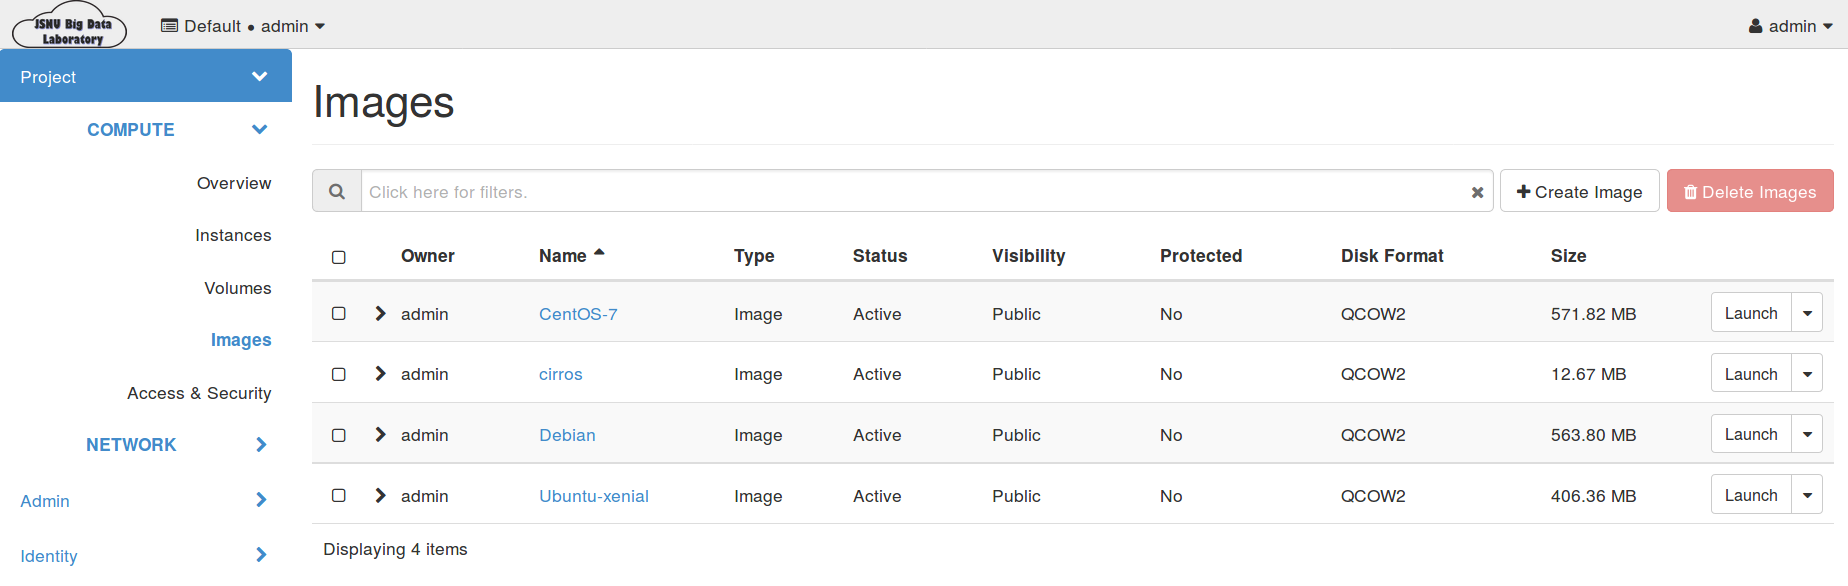
\includegraphics[width=6in]{./figures/Project_Compute_Images}
\caption{协作平台镜像管理}
\label{fig:projectcomputeimages}
\end{figure}
``Access \& Security''显示访问对象的安全相关信息。``Security Groups''列出了当前平台组信息,不同组拥有不同访问权限,用户可以通过右侧``Manage Rules''管理安全规则;``Key Pairs''现实系统中密钥管理信息,例如键值对,用户可以通过``+Create Key Pair''创建密钥管理信息,也可以通过``Import Key Pair''导入已有密钥信息。
\begin{figure}[!htb]
\centering
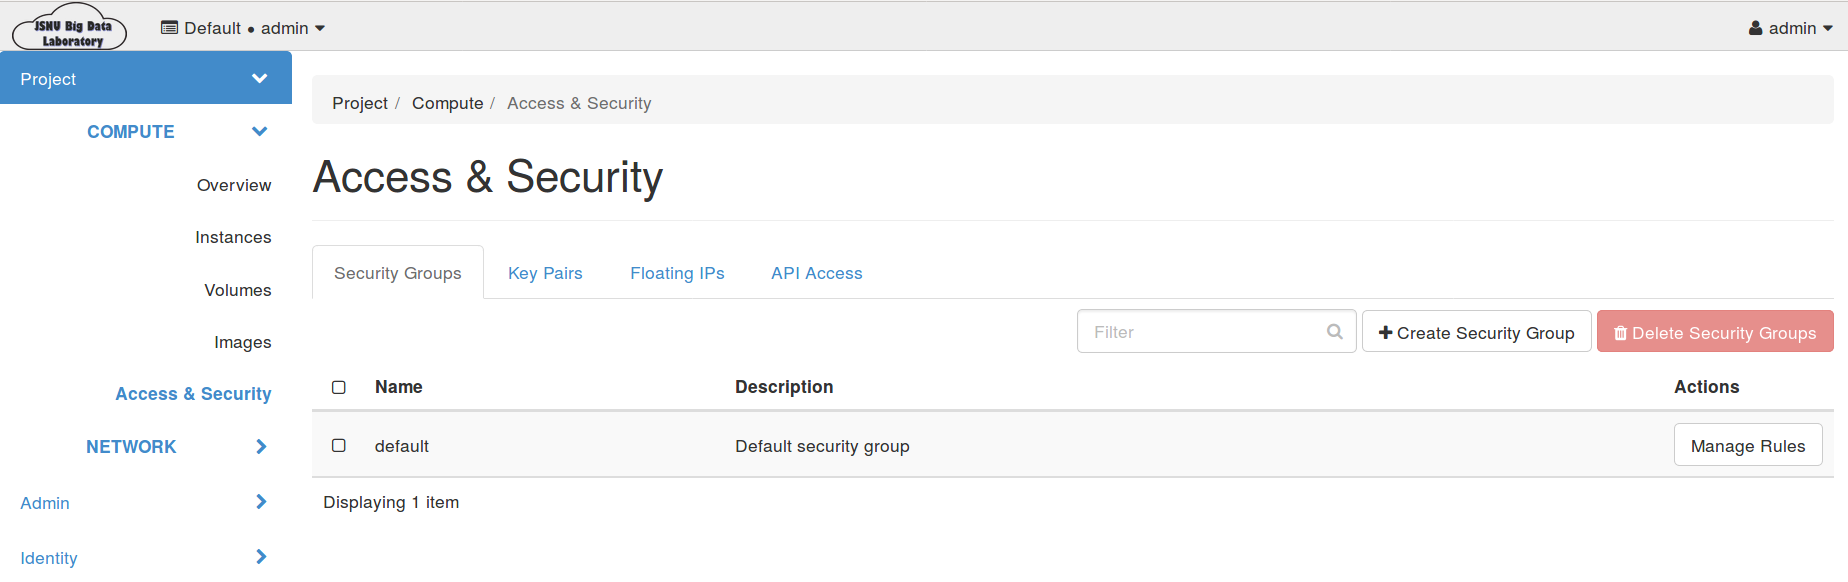
\includegraphics[width=6in]{./figures/Project_Compute_AccessSecurity}
\caption{协作平台安全管理}
\label{fig:projectcomputeAccessSecurity}
\end{figure} 
\section{协同计算大数据开发环境} 

%\section{协同计算并行管理系统}

\section{协同计算大数据架构系统}

\section{协同计算并行随机存储系统}
``Volumes''如图\ref{fig:projectcomputevolumes}显示卷管理信息;``Volume Snapshots''显示了卷快照信息。
\begin{figure}[!htb]
\centering
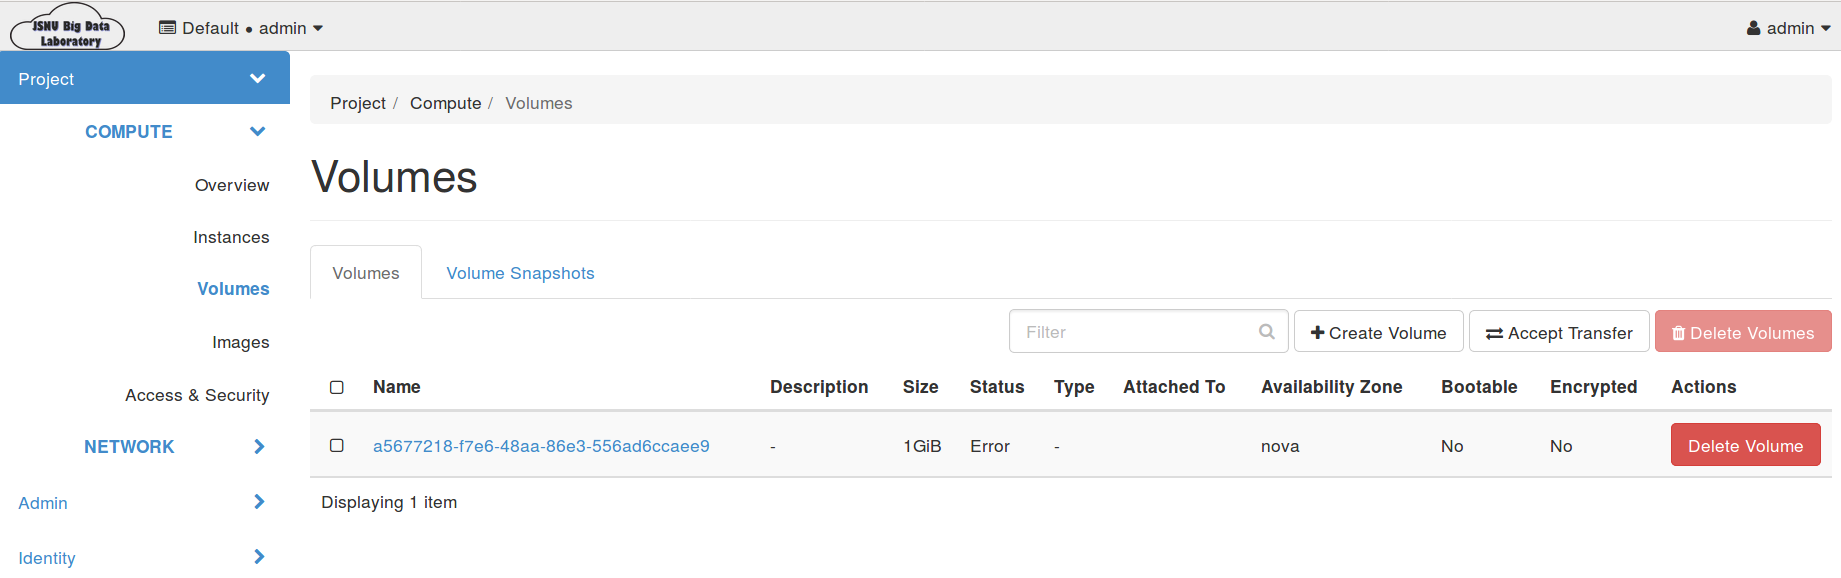
\includegraphics[width=6in]{./figures/Project_Compute_Volumes}
\caption{协作平台卷管理}
\label{fig:projectcomputevolumes}
\end{figure}
\section{协同计算网络环境系统}
``Network''集中展示了系统网络相关信息,如网络拓扑、路由等。如图\ref{fig:projectnetworktopology}显示了当前写作平台的网络拓扑结构,``Networks''如图\ref{fig:projectnetworknetworks}列出了平台网络出口信息。
\begin{figure}[!htb]
\centering
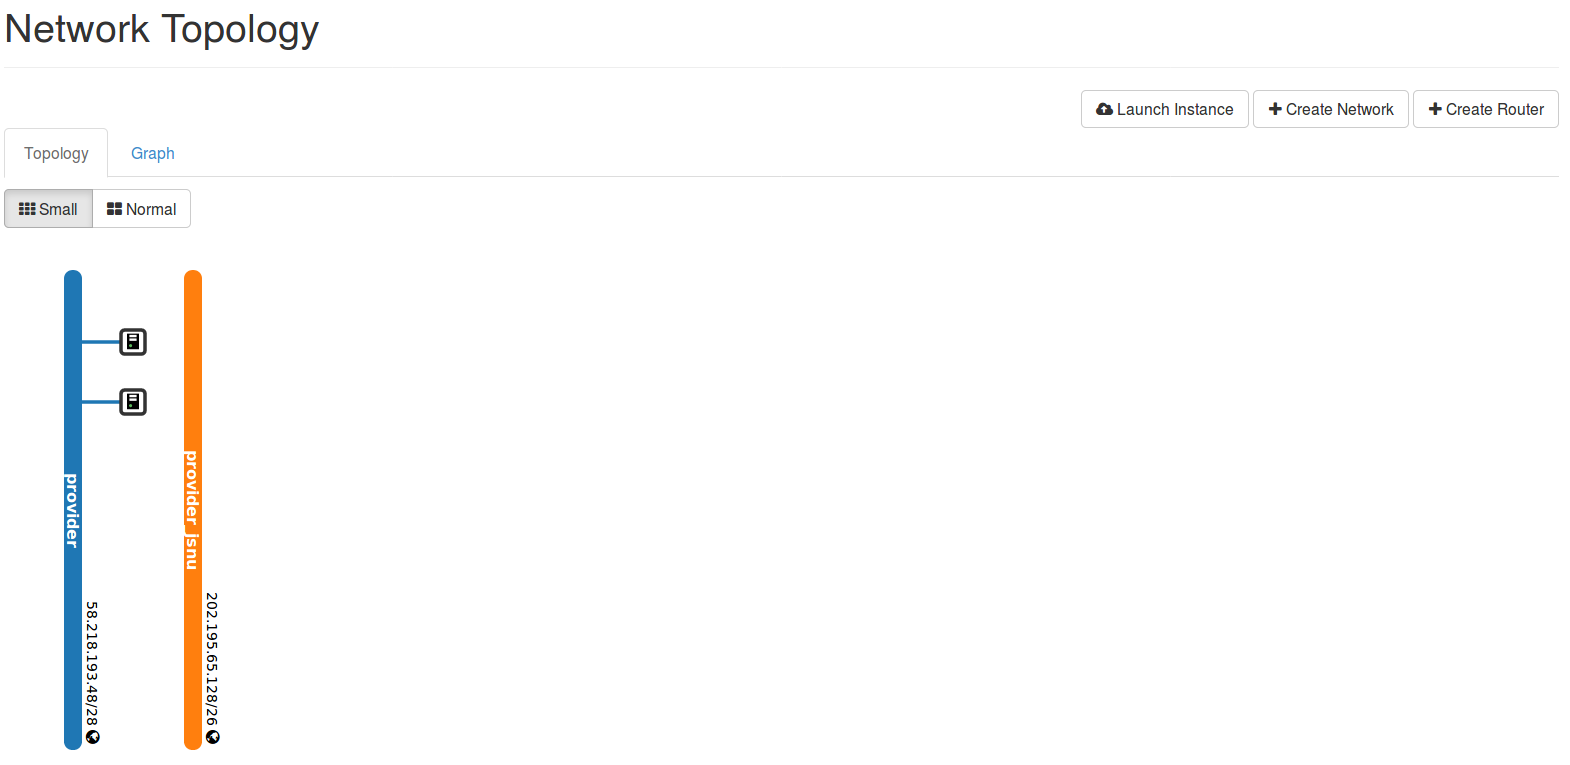
\includegraphics[width=6in]{./figures/Project_Network_Topology}
\caption{协作平台网络拓扑管理界面}
\label{fig:projectnetworktopology}
\end{figure}

\begin{figure}[!htb]
\centering
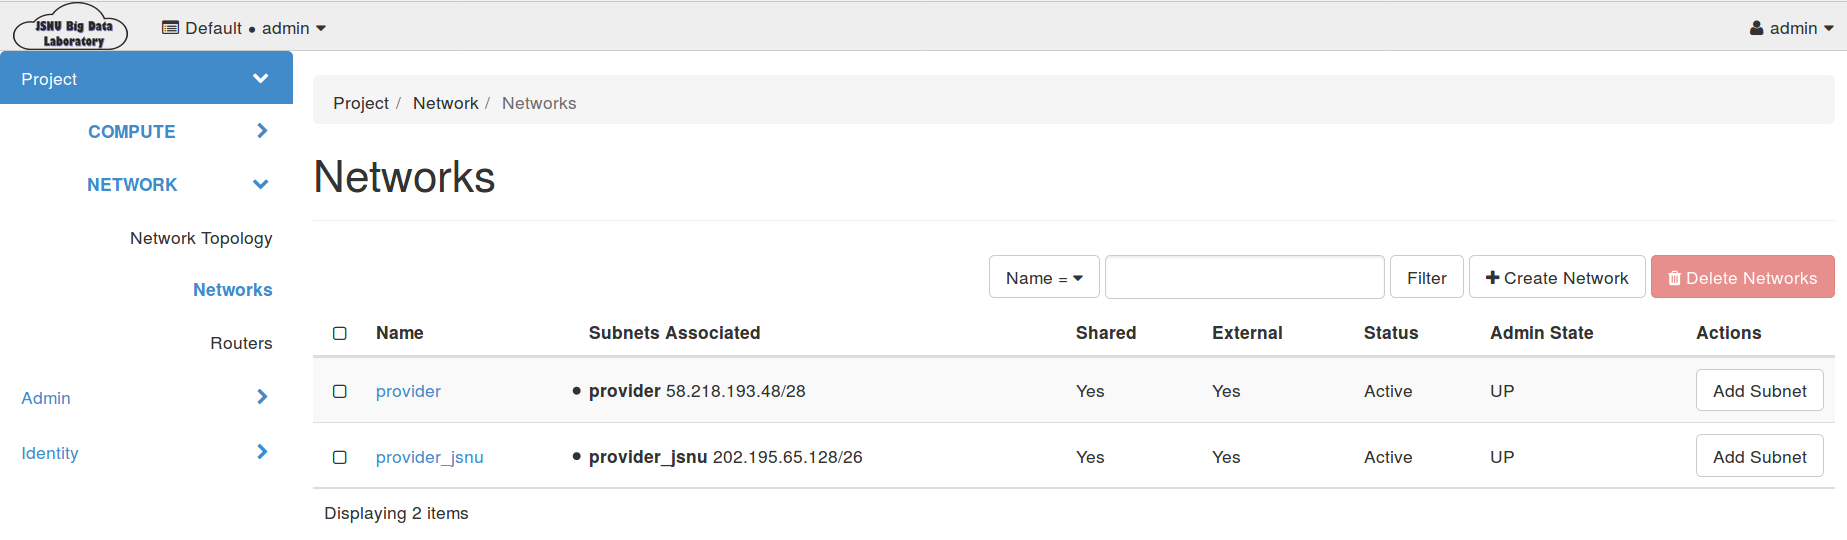
\includegraphics[width=6in]{./figures/Project_Network_Networks}
\caption{协作平台网络信息}
\label{fig:projectnetworknetworks}
\end{figure}





\section{使用指南}

\subsection{标识}
标识部分集中展示了项目、用户、群组以及角色等信息。图\ref{fig:identityprojects}所示给出项目标识包括的信息。项目标识列表显示所有当前运行在该协作计算平台的项目信息,如项目名称、项目描述、项目ID、运行状态等。另外,项目标识页面还提供创建项目、管理项目等功能,用户可以通过“+Create Project”按钮创建新项目,也可以在对应项目行最右侧“Manage Members”下拉菜单管理已有项目,例如删除项目、编辑项目、查看项目使用情况以及为该项目修改配额等。当写作平台运行项目数量较多时,用户也可以通过\ref{fig:identityprojects}页面上方的“Filter”设置特定规则,选择性显示部分项目。
\begin{figure}[!htb]
\centering
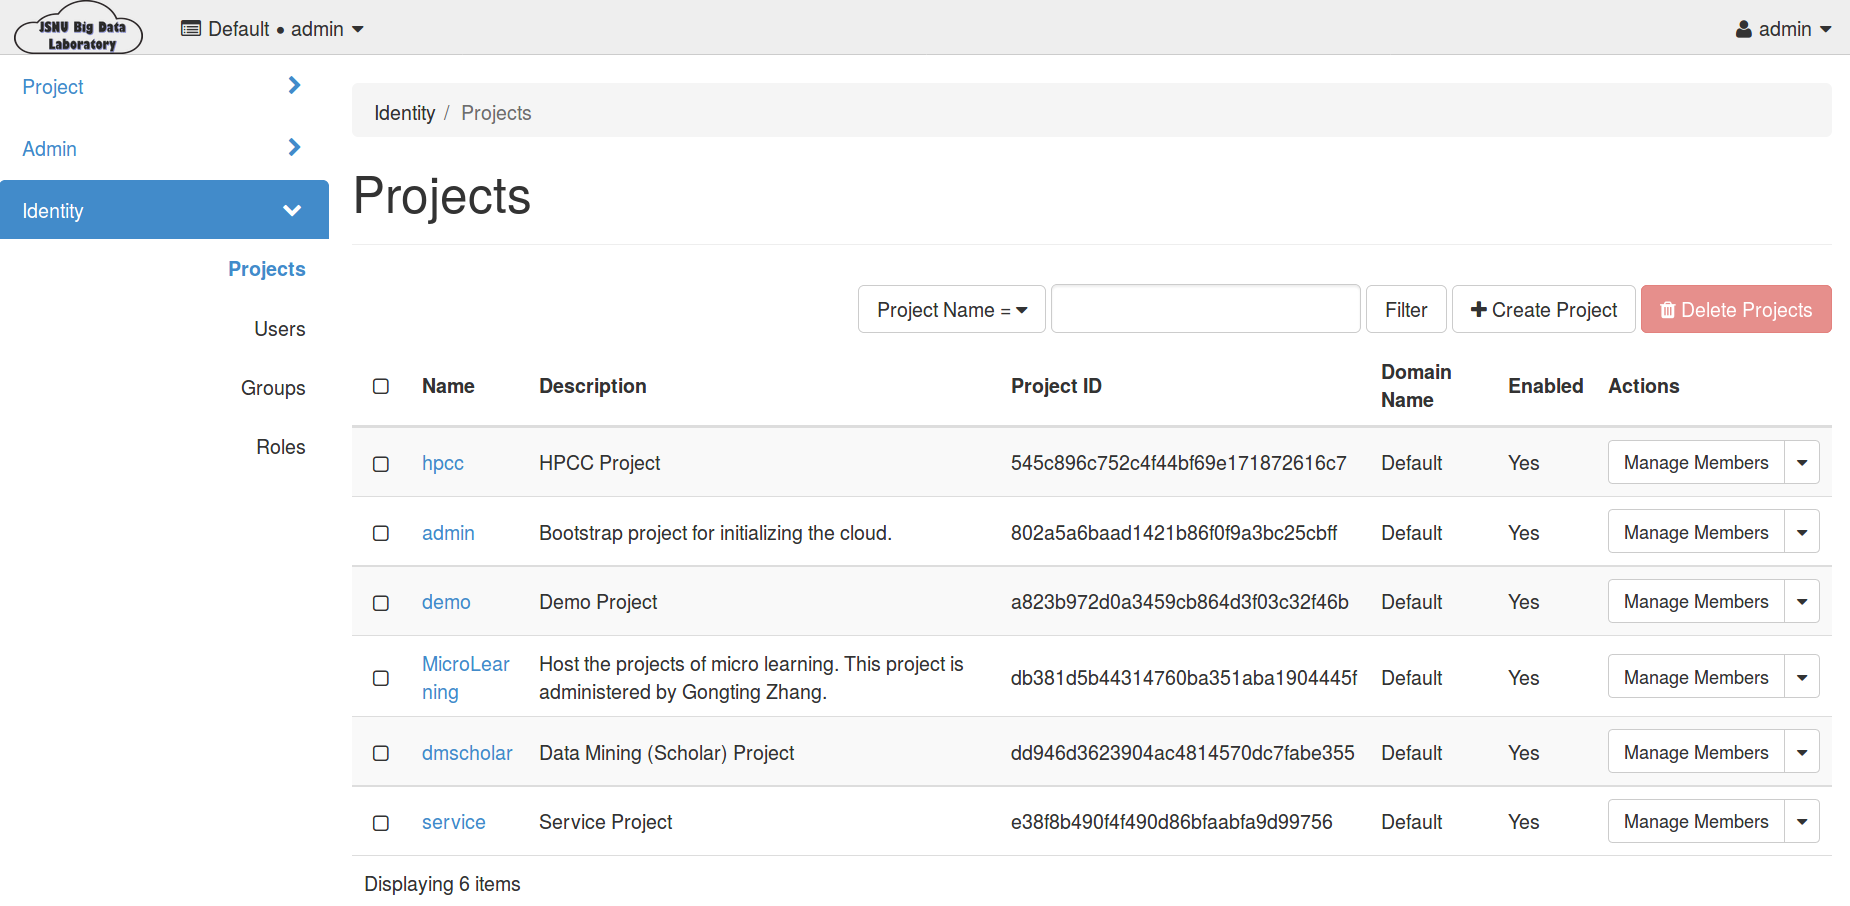
\includegraphics[width=5in]{./figures/Identity_Projects}
%\includegraphics[height=2.1338in, width=3.3307in]{./the_directed_neighbor_tree.png}
%\epsfig{file=./Fig1.png,height=2.1338in, width=3.3307in}
\caption{项目标识界面}
\label{fig:identityprojects}
\end{figure}





\subsection{项目}



\end{document}
